\documentclass[12pt,twoside,a4paper]{article}
\usepackage{lipsum}
\usepackage{setspace}
\usepackage{multirow}
\usepackage{tabularx}
\usepackage{graphicx}
\usepackage{amsmath}

\setlength{\parindent}{0pt}

\title{A Test \LaTeX\ Document}
\author{Martin Chorley}
\date{February 2013}
\begin{document}

\maketitle

\begin{abstract}
\lipsum[2]
\end{abstract}

\section*{Introduction}
\onehalfspacing
{\Huge Hello World!} This is       my       first       \LaTeX\     document.
This is not a new paragraph.

\textsc{This is a new paragraph.}

"Here is something in quotation marks"

``Here is something with grave accents and apostrophes''

\begin{center}{\tiny Here is some centred text}\end{center}

\begin{itemize}
	\item A list item
	\item Another item
	\item Some more item
	\item The end of the list
\end{itemize}

\begin{enumerate}
	\item First item in our list
		\begin{enumerate}
			\item First item in the sub-list
			\item Another item
					\begin{itemize}
						\item First item in the sub-sub-list
						\item Another item
							\begin{enumerate}
								\item First item in the sub-sub-list
								\item Another item
							\end{enumerate}
					\end{itemize}
		\end{enumerate}
	\item Yet more list items
	\item And one for luck
\end{enumerate}


\lipsum[1-4]

\section{Related Work}
\singlespacing

\lipsum[5-6]

\section{Tables}

Some tables

\vspace{0.2in}

\begin{tabular}{| r | c |}
\hline
first cell & second column \\
\hline
second row & last cell \\
\hline
\end{tabular}

\vspace{0.2in}

\begin{tabular}{ | r | l | }
    \hline
    \multicolumn{2}{|c|}{Table Heading} \\
    \hline
    some text & other text \\
this text & more text \\
    \hline
\end{tabular}

\vspace{0.2in}

\begin{tabular}{ | r | c | l | }
    \hline
    \multicolumn{3}{|c|}{Table Heading} \\
\hline
    \multirow{2}{*}{this text} & some text & other text \\
     & more text & other more text \\
    \hline
\end{tabular}

\vspace{0.2in}

\begin{tabularx}{\textwidth}{ | X | X | X | }
    \hline
    \multicolumn{3}{|c|}{Table Heading} \\
\hline
    \multirow{2}{*}{this text} & some text & other text \\
     & more text & other more text \\
    \hline
\end{tabularx}

\section{Images}

\setlength\fboxrule{6pt}
\setlength\fboxsep{0pt}
\fbox{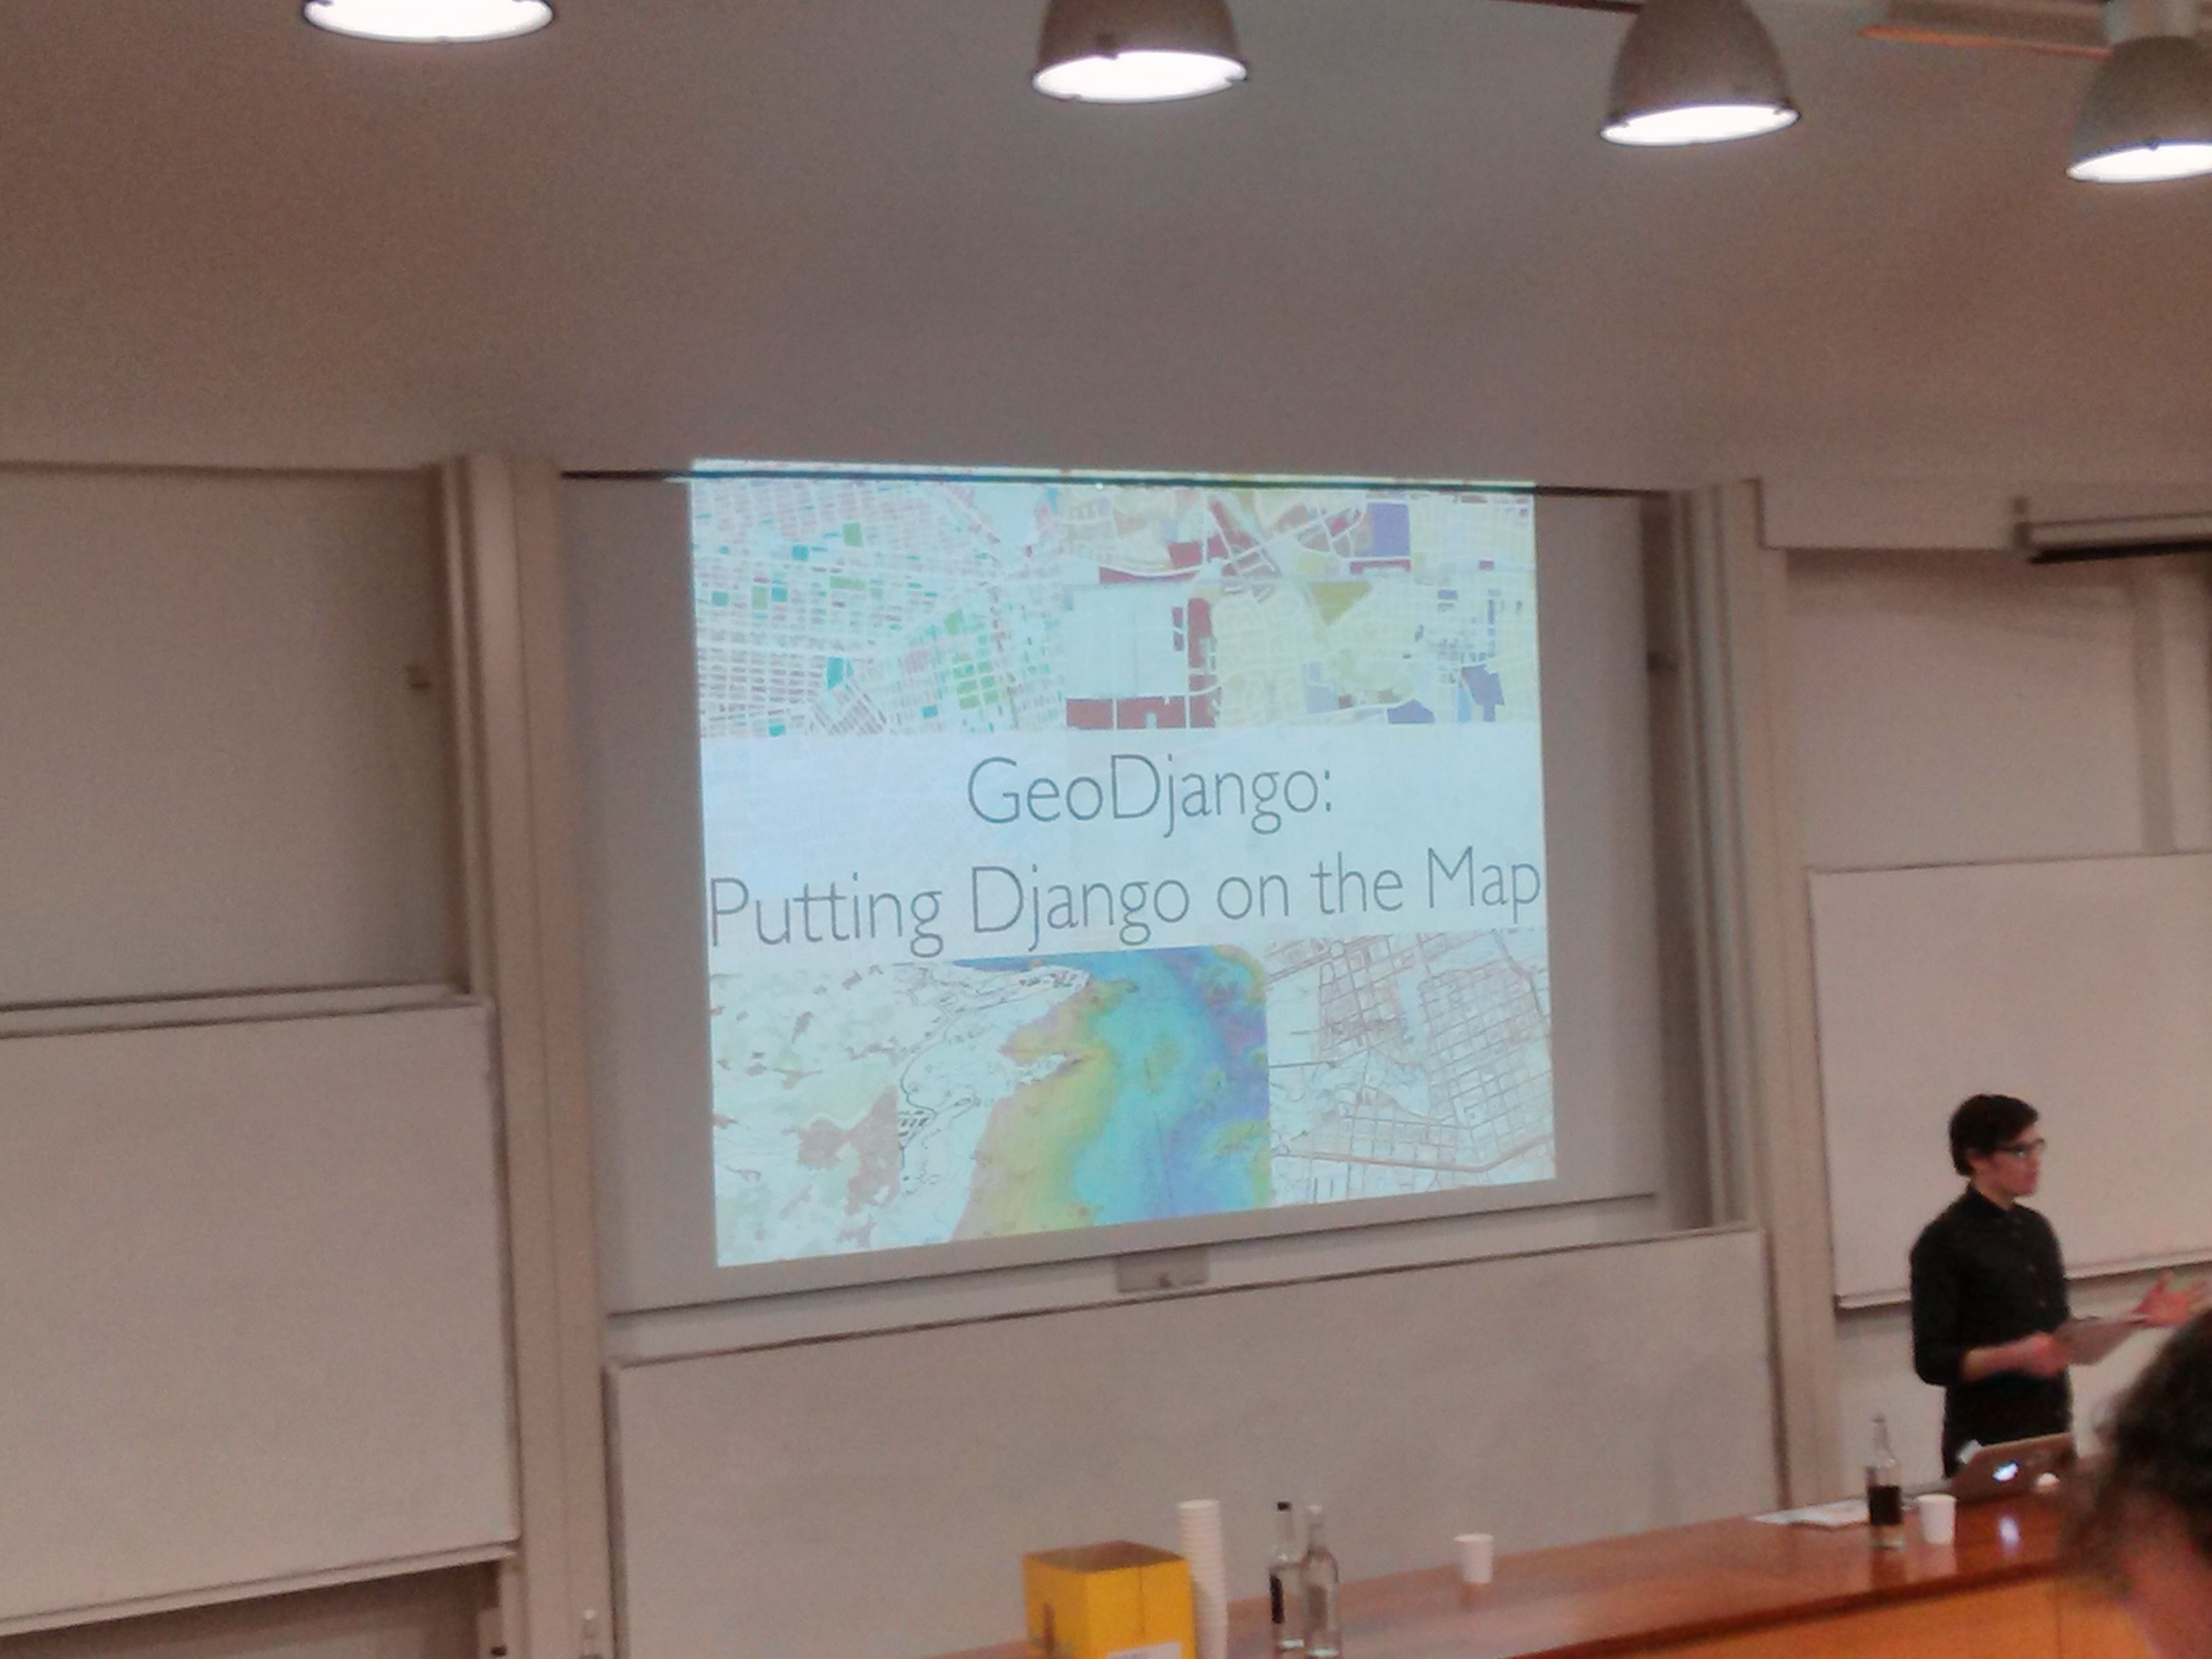
\includegraphics[width=0.5\textwidth]{img/django.jpg}}


\[ \int_0^\infty x^2\,dx \]

\[ \int_0^\infty x^2\,\mathrm{d}x\]

\[  \left(\frac{x^2}{y^3}\right) \]

\[ \Bigg[ 0\Bigg] \]

\[ [ 0 ] \]

\[ 50 \text{ apples} \]
\end{document}